\section{Performances} % (fold)
\label{sec:perf}

Les tests de performances ont été effectués sur la machine PlaFRIM, en utilisant 4 noeuds et 4 processeurs par noeuds.

La première version du code améliorée avec \texttt{OpenMP} donne des résultats intéressants, mais possibles à améliorer. Quand les blocs deviennent très grands les accès mémoire ralentissent le programme. L'idée est de séparer les calculs en blocs (pavage) pour réduire ces temps d'accès à la mémoire (seconde version \texttt{OpenMP}). Les tailles des blocs doivent être calées exactement sur la taille du cache. Une mauvaise taille entraîne une perte de performance, comme on peut le voir sur la figure \ref{fig:sp-thread}, où la taille des blocs était de $64$. Une autre possibilité disponible avec \texttt{OpenMP} est l'utilisation des tâches. On génère des tâches ayant des tailles de blocs optimales et on exécute ces tâches. Un des avantages d'\texttt{OpenMP} est de pouvoir définir facilement un nombre de threads quelconque.\\

Pour les performances obtenues avec \texttt{pthread}, elle sont similaires à \texttt{OpenMP} pour le même nombre de threads. En effet, les deux versions utilisent le même type de ressources pour améliorer le temps de calcul. Le programme \texttt{pthread} actuel utilise des barrières pour s'assurer que les calculs précédents ont été effectués (à la façon d'\texttt{OpenMP}). Il est possible, avec un sémaphore par thread, de limiter les attentes à la terminaison des blocs adjacents et ainsi pour voir commencer l'étape suivante alors que certains threads n'ont pas terminé la précédente. Comme le nombre de threads disponibles sur un processeur ne peut pas dépasser une certaine valeur, il est plus intéressant (dans le cas des sémaphores) d'utiliser des blocs colonnes (car les matrices sont stockées en colonne dans notre projet). Enfin les blocs de threads ayant une taille dépendant de la matrice, il faudrait découper ces blocs en sous-blocs pour pouvoir optimiser les accès à la mémoire.


\begin{figure}[!ht]
\centering
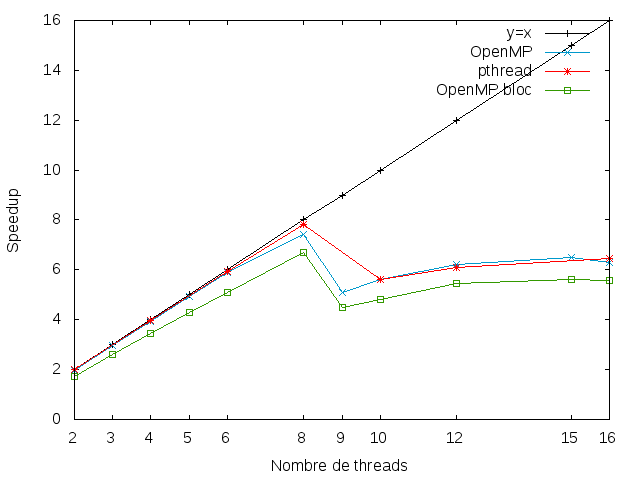
\includegraphics[width=0.8\textwidth]{speedup-thread.png}
\caption{Speed up des versions à mémoire partagée}
\label{fig:sp-thread}
\end{figure}

La figure \ref{fig:sp-thread} montre les résultats obtenus pour les versions à mémoire partagée (OpenMP et pthread) en faisant varier le nombre de threads.


Les performances de la version \texttt{MPI} sont meilleures que celles des versions multi-thread. \texttt{MPI} permet rajouter un nombre illimité de processus et donc de dépasser les accélérations des autres versions. Les trois versions de \texttt{MPI} ont des performances sensiblement identiques car les matrices testées ne sont pas exceptionnellement grandes et le nombre de processus reste relativement faible comparé à un gros calculateur. Cependant, la version synchrone avec les communications bloquantes reste la moins efficace, puisqu'elle ne fait rien durant ses communications. La différence entre la version asynchrone et la version persistante est la rapidité d'exécution des communications. La version persistante n'a pas besoin de copier les buffers et de préparer les requêtes ; le programme gagne donc un peu de temps, mais cela n'est visible que sur de longues exécutions avec beaucoup de communications.

\begin{figure}[!ht]
\centering
% \includegraphics[width=0.8\textwidth]{sp-proc.png}
\caption{Speed up des versions multi-processus}
\label{fig:sp-proc}
\end{figure}

La meilleure solution est de combiner \texttt{MPI} avec \texttt{OpenMP} ou \texttt{pthread} pour multiplier les gains de performance, puisqu'un processus \texttt{MPI} s'exécute sur un c\oe ur qui peut avoir plusieurs threads.


\section{Discussion} % (fold)
\label{sec:discussion}

Le sujet évoquait le problème de charge inégale des calculs. En effet, dans certaines zones du plateau de jeu, il peut y avoir très peu de calcul. Lorsque, entre deux pas de la variable $loop$, il n'y a pas de changement pour une zone, on sait que celle-ci ne changera plus tant que ses bordures ne changent pas (donc lors d'échanges avec ses voisins). Cela permet d'effectuer un peu moins de calcul.

Cependant, dans notre implémentation actuelle, toutes les zones sont censées être calculées en parallèle. Et dans ce cas, qu'une zone ne travaille pas alors que ses voisins travaillent ne change rien en terme de temps d'exécution, bien que certains processus puissent se ``reposer'' un peu. 

Si les processus et leurs threads pouvaient se répartir mieux la charge de travail, on pourrait par contre gagner en performances. Plusieurs procédés existent pour cela, que nous avons pu voir au travers des différents TDPs. Le vol de travail permettrait aux processus inactifs de faire quelque chose au lieu d'être inactif, tout en réduisant la charge de travail d'un autre. 

Dans les versions \texttt{MPI} que nous avons écrites, les processus ne contenaient qu'une zone à calculer, comme cela était demandé par le sujet. Il serait probablement plus intéressant de donner plusieurs zones du plateau à chaque processus. Celui-ci se chargerait ensuite de les calculer, en les répartissant par exemple parmi ses threads. 

Il est probable qu'une zone où il ne se passe rien sur un long moment soit au milieu d'une plus grande zone inactive. Dans ce cas, si un processus contient toutes ces zones connexes inactives, il ne fera rien tandis que les autres processus travaillent.

Dans le cadre de cette idée, au lieu de répartir les processus sur une grille de façon ``linéaire'', nous pourrions utiliser une répartition en serpentin, ou en bloc-cyclique, afin de pallier le problème. Il est possible aussi d'utiliser une répartition pseudo-aléatoire, par exemple en usant du théorème de restes chinois. Les zones inactives seront alors bien réparties entre les processus. Un processus aura donc plus de chance d'avoir du travail. 

